\documentclass[thesis.tex]{subfiles}
\begin{document}

\chapter{Main}\label{chap:basics}

\section{Overview}
Inspired by Lensing's LightSkin approach~\cite{bib:LightskinPaper}, we want to compute indirect lighting only at specific locations and interpolate the results over multiple pixels, as opposed to techniques like Reflective Shadow Maps or Voxel Cone Tracing.
Like other previous works, we call these locations \emph{Light Caches}.

\begin{figure}[h]
	\centering
	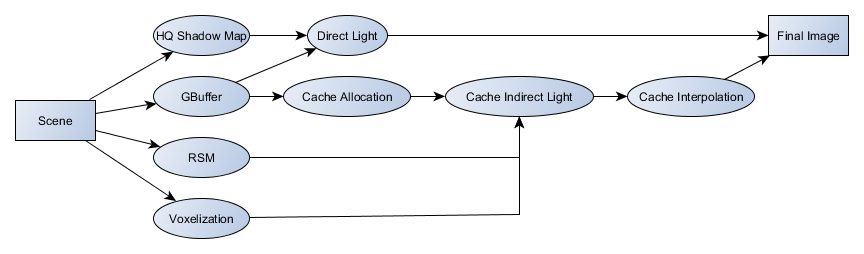
\includegraphics[width=\textwidth]{renderingpipeline_draft}
	\caption{Overview over our basic rendering pipeline.}
	\label{fig:pipelineoverview}
\end{figure} \todo{Add Images?}
Our technique consists of three basic steps which are executed in every frame: Cache allocation, indirect lighting and cache interpolation.
\autoref{fig:pipelineoverview} gives an overview of the pipeline steps and their dependencies.
The cache allocation pass assigns cells on a regular grid to cache memory, thus creating the caches that are about to be used in this frame.
Using a reflective shadow map, indirect lighting is then computed for all caches.
Finally each pixel interpolates an indirect lighting value using all neighboring caches within the grid.

Each of the following major sections will explain one of these stages and their interdependencies.
The last major section of this chapter will elaborate several implementation details, some of them crucial to the overall performance.\\
Many parts of our approach are based on several well-known techniques of which most have already been discussed in \autoref{chap:prevwork} and \autoref{chap:basics}.
Where necessary, details of the respective algorithms will be elaborated to address specifics implied by the overall technique.

\section{Cache Allocation}
Since the goal of this work is a fully dynamic solution that works without any pre-computations, it is necessary to place all caches at runtime, as opposed to LightSkin~\cite{bib:LightskinPaper} where caches are placed in a computational intense preprocessing step.
Instead, we use a grid based approach similar to Vardis et al. \cite{bib:radiancecachechromaticcompression}.
Before we discuss the details of our solution, several general implications of such an approach are elaborated.

\subsection{General Properties of Dynamic Cache Placement} \label{sec:impl:dyncacheplace}
Compared to a precomputation based approach, there are several intrinsic advantages which can be expected of a dynamic light cache placement.
Since we try to achieve only a single bounce of indirect light, caches are only used by locations that lie in the current view frustum. % (for multiple bounces however, it might be necessary to transfer lights between caches).
It should be possible to decrease the number of caches for distant objects, thus keeping screen-space cache density within a given bound.
%Both properties result in a much lower memory footprint especially for large scenes.
\\
While it can be very beneficial to place caches entirely dependent on view space informations, this also may introduce several temporal artifacts if caches disappear or move, i.e. strong changes in indirect lighting from one frame to the next.
Additionally, it is necessary to guarantee that target pixels have easy access to a certain number of caches to be able to interpolate them.
Note that the interpolation pass can have temporal coherence problems on its own, as the assignment of a cache to its surrounding world positions needs to be stable, no matter how densely they are sampled, i.e. how many pixels a given world space area covers.

%So far, the data requirements of each cache have not been defined yet.
Precomputed caches can naturally hold almost arbitrary data. % (as long as a given memory bound is not exceeded).
Dynamic caches on the other hand need to acquire their data every frame, which is not only costly performance-wise but may also cancel out certain types of data as it may not be accessible.
For example LightSkin~\cite{bib:LightskinPaper} needs to a rather complex area metric for each cache that can not be computed in real-time.
Naturally, such constraints also affect the following lighting and interpolation stages tremendously.

We evaluated several approaches before we came up with our final algorithm.
If you are interested you can read the summary of these attempts in \autoref{chap:abandoned}.

\subsection{Cache Address Volume}
\begin{figure}[h]
	\centering
	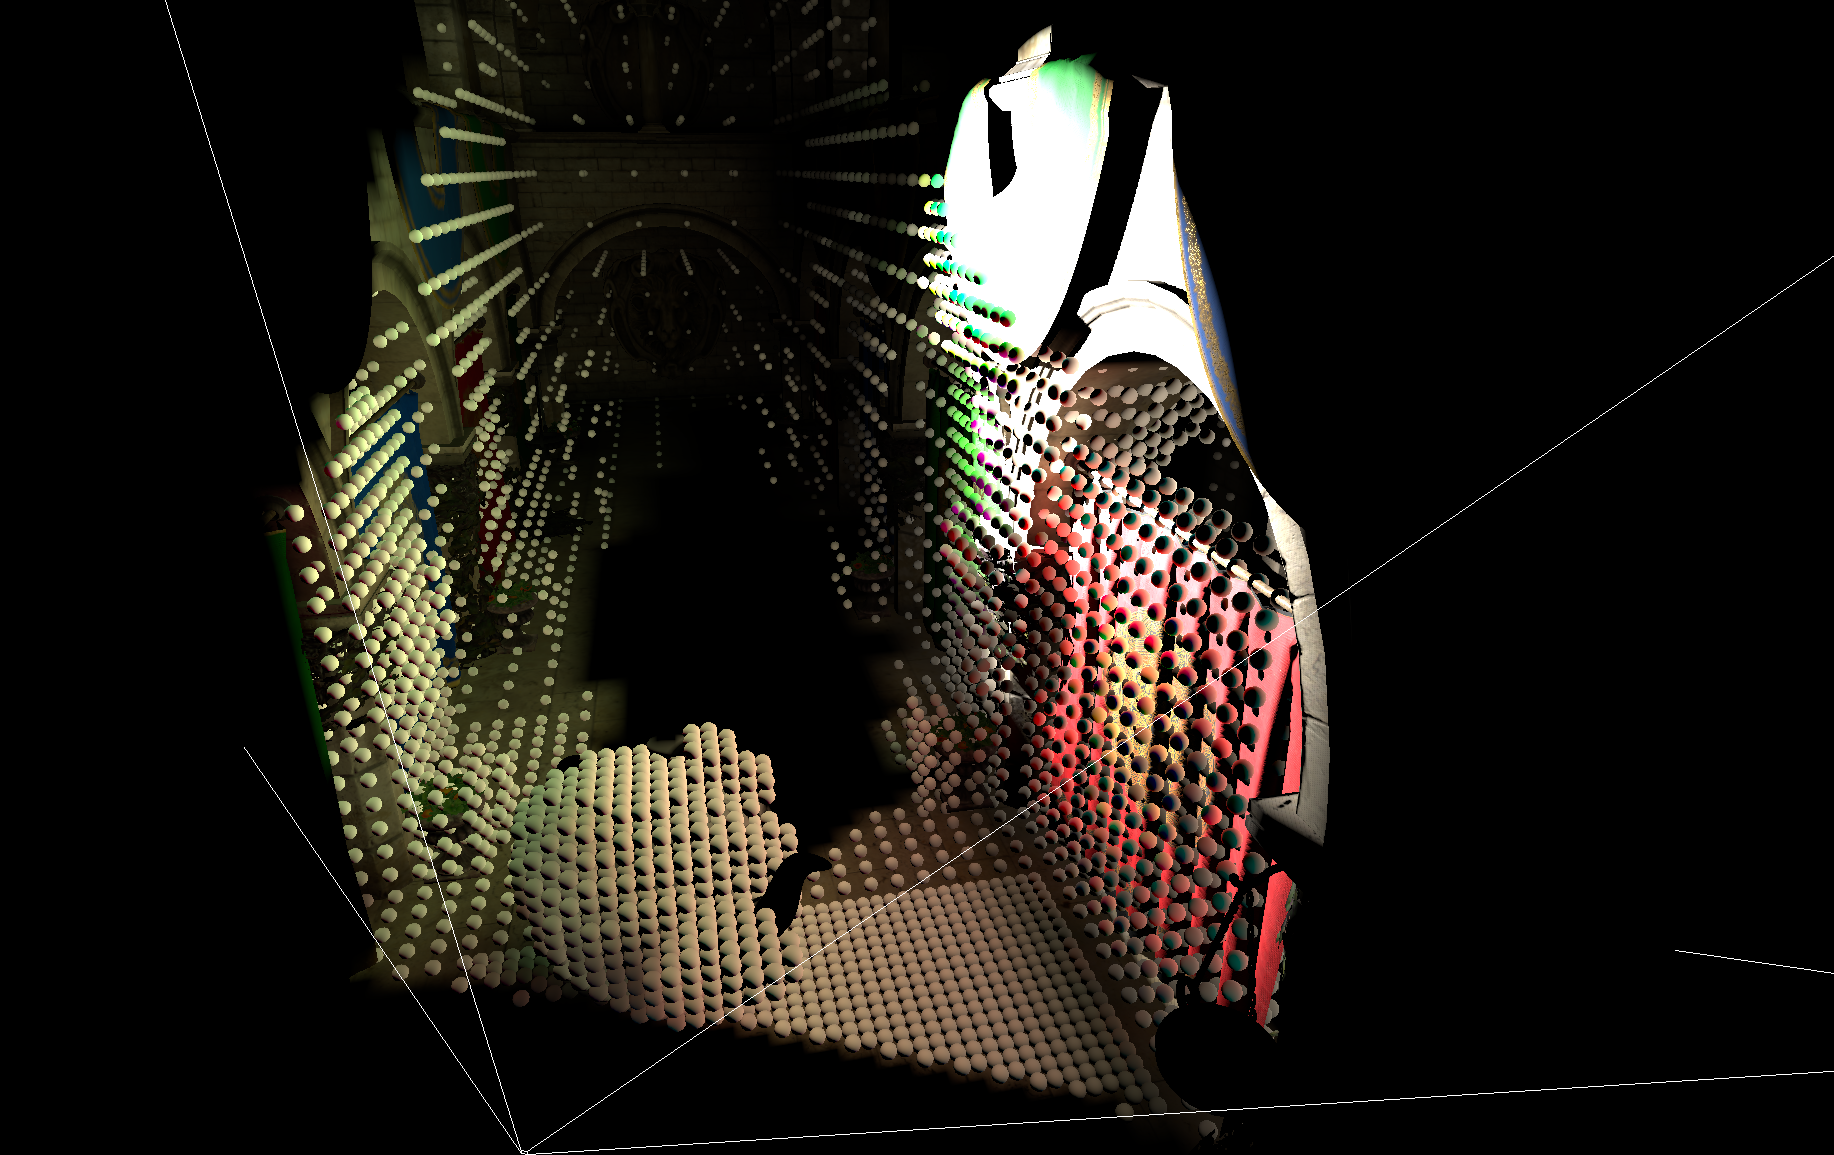
\includegraphics[width=\textwidth]{cachevis}
	\caption{Visualization of active caches for a view hinted by the white lines. Note that there is a "shadow" behind the object in the middle where no caches are active since the camera can not see behind it.} \label{fig:cachevis}
\end{figure}
To cancel out temporal artifacts entirely, we decided to place caches only at the nodes of a regular world space grid.
The main disadvantage of this method is, that caches are not placed on surfaces and thus can not have a specific orientation.\\
Since only a small fraction of all grid cells contains any caches, they are stored in a separate buffer and only their addresses are saved in the grid.
Accordingly, we call this grid the \emph{Cache Address Volume (CAV)}.
This approach reduces not only the memory consumption drastically, it makes it also much easier to perform the lighting for each cache, as they lie now consecutive in memory instead of being scattered within a volume as in Vardis et al. \cite{bib:radiancecachechromaticcompression}.

During the cache allocation pass the CAV is cleared and then refilled depending on the current view.
This is done by a full-screen pass, using the per-pixel world-positions from the previously rendered scene. % (which can be acquired using the depth buffer).
Each pixel allocates caches at the eight nearest CAV cells.
If an affected cell already contains a valid cache address, it is skipped as pixels do not introduce any data besides the cache allocation itself.
Since neighboring pixels often access the same grid cells, there is room for some optimizations using shared memory which are explained in \autoref{sec:impl:cachealloc}.
\autoref{fig:cachevis} shows a resulting cache distribution.

\subsubsection{Cascading} \label{sec:impl:cavcascading}
\begin{figure}[h]
	\centering
	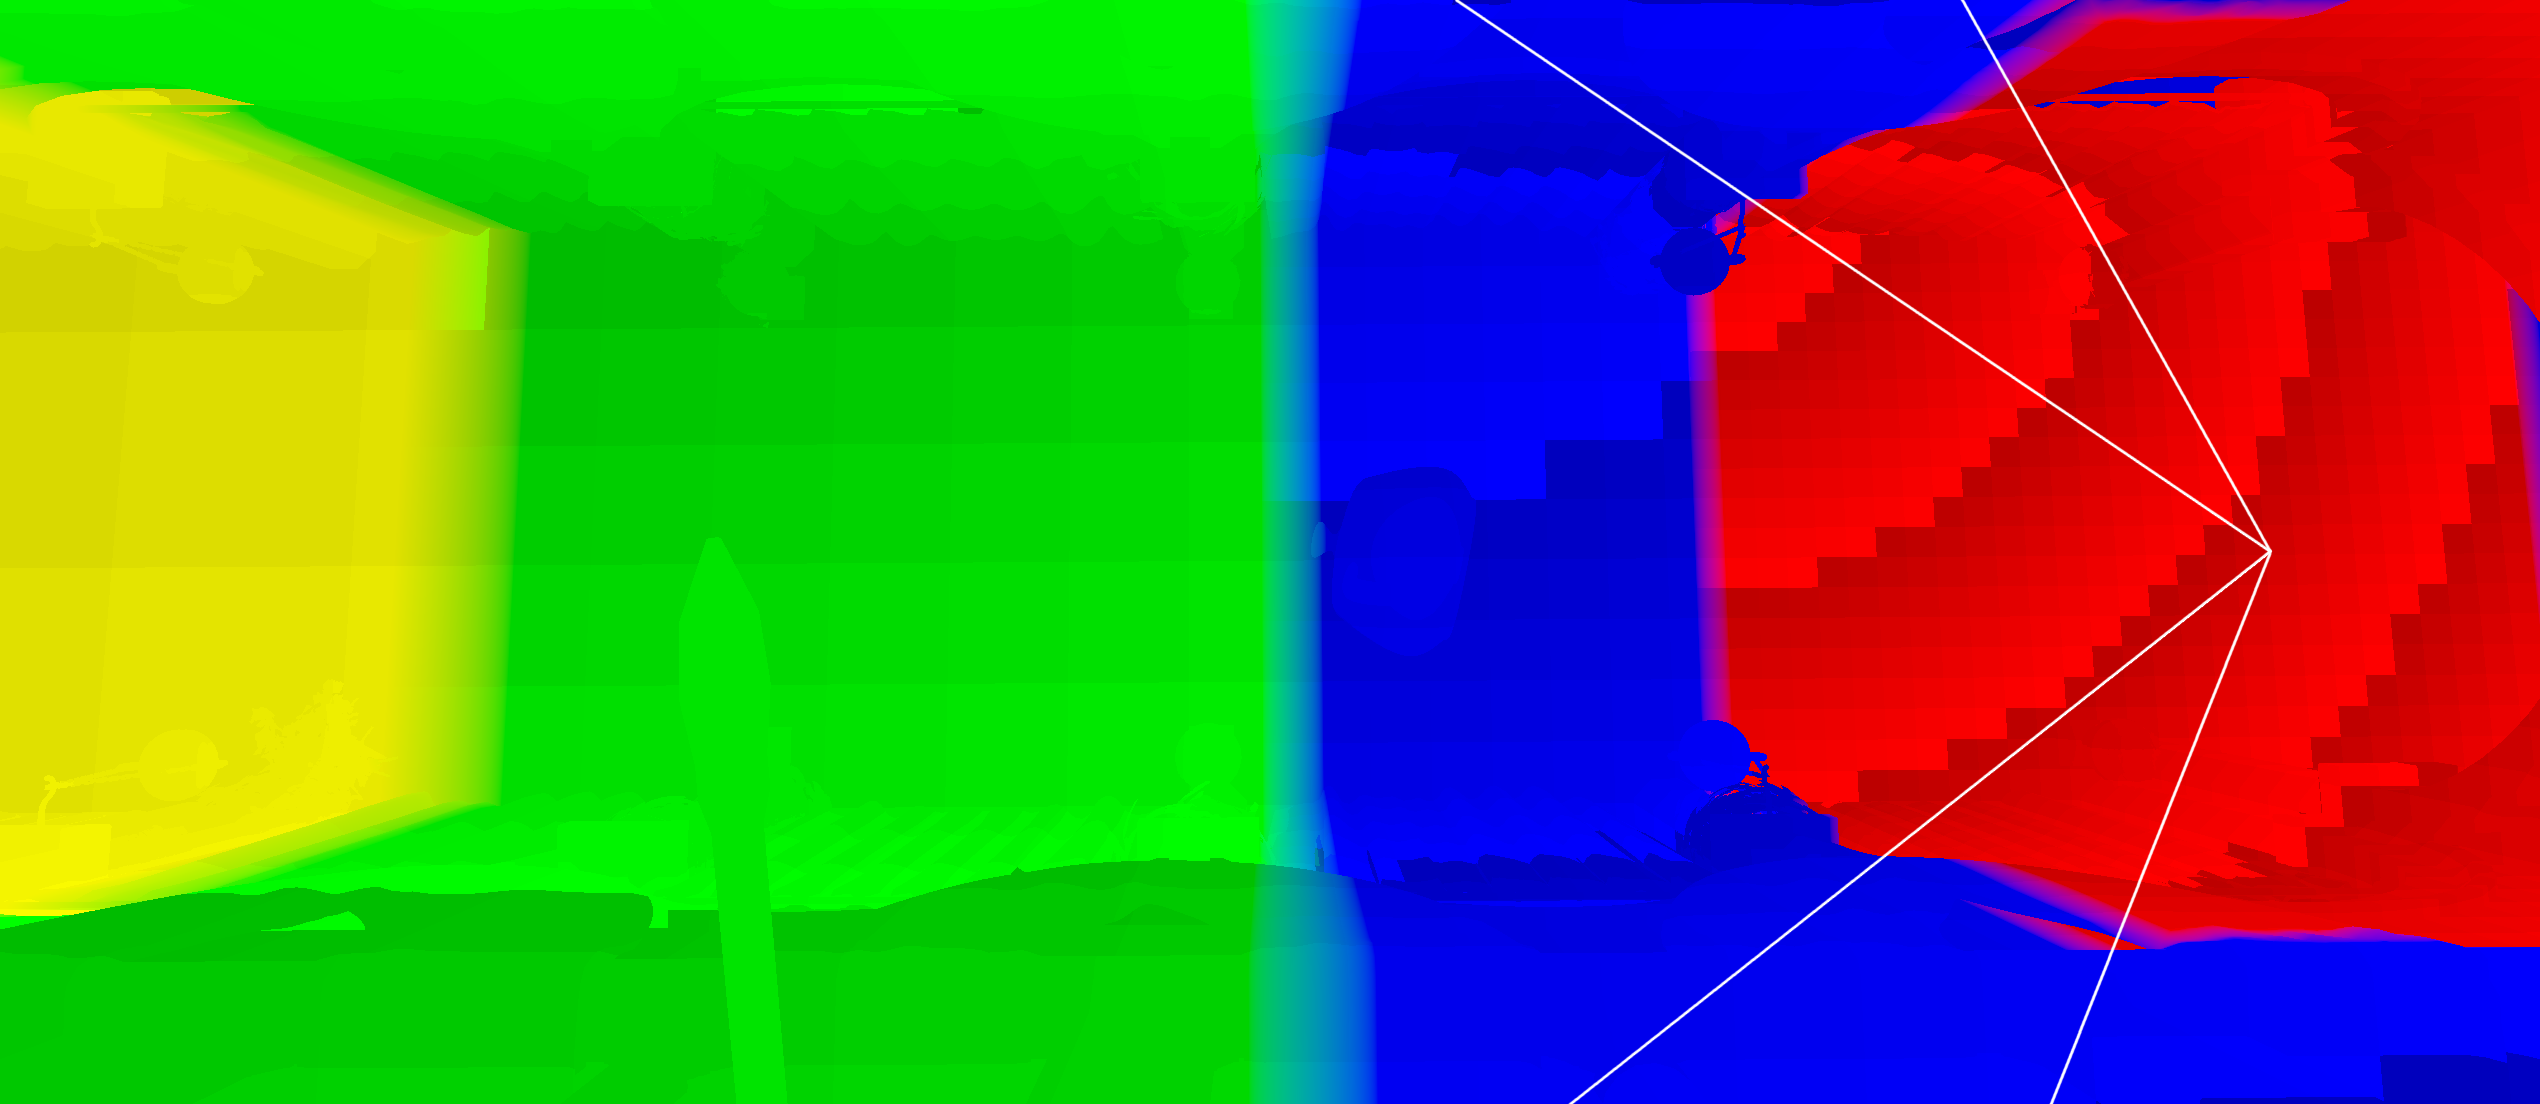
\includegraphics[width=\textwidth]{cascades}
	\caption{Visualization of CAV cascades. Again, the white lines to the right show the active view frustum. The brightness differences within a cascade (single colored area) hint the cache size.} \label{fig:cavcascades}
\end{figure}
Similar to Cascaded Light Propagation Volumes \cite{bib:lpt} a set of nested CAV cascades are centered around the camera.
\autoref{fig:cavcascades} visualizes the cascading system.
This introduces a distance dependent level of detail and keeps the number of caches constant, even for large scenes.
The cascade positions are snapped to multiples of their grid size to ensure consistent lighting results. %\todo{elaborate the snapping-whys further?}
For simplicity, all CAV cascades are cubic and have the same resolution, while their grid size is doubled for each consecutive cascade.

Caches are only allocated in the smallest CAV cascade which encloses a given pixel world-position.
To be able to allocate all eight nearest CAV cells in a single cascade, special "decision boundaries" which are smaller than the actual cascade are used for cascade selection.
As the snapped movement introduce temporal incoherency, we move the decision boundaries smoothly with the camera and shrink them further by another grid cell size to ensure that they are fully enclosed by their respective cascades.
\\
Additionally, there are transition areas between two successive cascades.
Within these areas, caches are allocated in both cascades to be able to avoid hard edges during the interpolation stage late on.
The size of the transition areas can be chosen freely.
For our demos we use transition areas as wide as twice the cell size of the smaller involved cascade.
This delivers sufficiently smooth transitions for reasonable performance costs in our scenes.

Contrary to Light Propagation Volumes, the cascades are not displaced with the view direction, but strictly centered around the camera position as this helps to keep the level of detail stable against view rotations.\\
While this means that a very large portion of each cascade is never used at all, the costs are still rather low since there are no computations involved for empty cells.
Also, the memory footprint is still rather small: %nevertheless
A high detailed setup consists of four cascades, each with a resolution of $64^3$.
With four byte address in each cell, this makes 4MB for all CAV cascades together.

\section{Indirect Lighting}
The indirect lighting of the caches relies on reflective shadow maps (see \todo{citation needed}).
In principle each cache iterates on the entire RSM to retrieve the encoded lighting informations.
The following chapters explain how this information is processed and how the results are saved for later interpolation.

\subsection{Diffuse Lighting} \label{sec:impl:diffuse}
We make use of the common separation of diffuse and specular lighting, making the later an optional feature that may be deactivated to save resources if necessary. \todo{principle should be in the basics chapter}
Diffuse lighting is comparatively easy to compute and represent since, for a given position and reflectivity, it is a low frequency function over a surface normal, independently of the view direction.

Recall the rendering equation for pure diffuse surfaces:
\begin{equation}
L_d (\mathrm{x}) = \frac{\rho_d}{\pi}\int\limits_{2\pi sr} L_i(x,\omega_i) \cdot \cos\theta \,\mathrm{d}\omega_i
\end{equation}
Using the reflective shadow map, an approximation of the integral can be expressed as a sum over $n$ virtual area lights:
\begin{align}
L_d (\mathrm{x})
&=\frac{\rho_d}{\pi}\sum\limits_{i=0}^{n} L_i \cdot (\hat{\mathbf{n}} \cdot \hat{\mathbf{d}}_i)^+ = \\
&=\frac{\rho_d}{\pi}\sum\limits_{i=0}^{n} \frac{I_i }{||\mathrm{x} - \mathrm{x}_i||^2 +  A_i} \cdot (\hat{\mathbf{n}} \cdot \hat{\mathbf{d}}_i)^+ \\
&=\frac{\rho_d}{\pi}\sum\limits_{i=0}^{n} \frac{\frac{\phi_i}{\pi} (\hat{\mathbf{n}}_i \cdot (-\hat{\mathbf{d}}_i) )^+}{||\mathrm{x} - \mathrm{x}_i||^2 +  A_i} \cdot (\hat{\mathbf{n}} \cdot \hat{\mathbf{d}}_i)^+
\end{align}
\todo{Where do we explain the disc light thing? Need to derive this formular much slower!}
%Each RSM pixel is interpreted as a disc-shaped light as described by Lensing (see \todo{either explain here or earlier}).

The diffuse reflectivity $\rho_d$ is usually given by a texture and varies per pixel.
However, since it is not part of the sum over all RSM pixels, it can be applied easily during the cache interpolation stage.\\
As caches are not placed on surfaces, there is no known normal vector $\hat{\mathbf{n}}$.
The only other quantity that does not depend on the RSM is the position, which is known for each cache.
Accordingly, each cache saves irradiance as a function over the normal vector.
We chose a low-order spherical harmonics representation to to approximate this function since it allows iterative computation and easy evaluation at runtime.\\ 
The irradiance contribution of a single light to the spherical harmonics coefficients can be derived analytically. \todo{put the meat of all this in prerequisites}
For a single light, the irradiance is symmetric to its direction.
Using this property, rotated Zonal Harmonic coefficients can provide an much easier way of deriving the irradiance contribution than directly using Spherical Harmonics.
First, Zonal Harmonic coefficients $z_l$ are computed for a fixed light direction, pointing to $(0,0,1)$.
\begin{align}
z_l =&\int\limits_{2 \pi sr} L_i \cdot (\omega \cdot (0,0,1))^+ \cdot y^0_l(\omega) \,\mathrm{d}\omega\\
=&\int\limits_{2 \pi sr} L_i \cdot \cos\theta \cdot y^0_l(\omega) \,\mathrm{d}\omega
\end{align}
Note that by integrating only over the upper hemisphere, the cosine does not need to be explicitly clamped.
Due to the rotation invariance of Spherical Harmonics, the resulting Zonal Harmonics coefficients can be rotated to the light direction (see \autoref{sec:preq:zonalharmonics}).
The resulting expressions for the first three SH bands can be found in \autoref{chap:shcosinelobe}.

To perform the diffuse cache lighting, the coefficients for all virtual lights are accumulated and saved into the cache buffer for later evaluation. \todo{add a note on how many bandy are required}

\subsection{Specular Lighting} \label{sec:impl:specenvmap}
As mentioned in \autoref{sec:preq:brdf} we make use of a normalized version of the Blinn-Phong BRDF.
Using virtual point lights from the Reflective Shadow Map, we define the specular part of the visible radiance is defined as following:
\begin{equation}
L_s (\mathrm{x}) = \rho_s \cdot \frac{\gamma + 8}{8\pi} \cdot \sum\limits_{i=0}^{n} ((\hat{\mathbf{n}} \cdot \hat{\mathbf{h}}_i)^+)^\gamma \cdot L_i \cdot (\hat{\mathbf{n}} \cdot \hat{\mathbf{d}}_i)^+
\end{equation}
%Since the view direction is fixed for a given frame, 
It would be possible to approximate the specular lighting via multiple sets of Spherical Harmonics coefficients similar as done previously for the diffuse lighting.
However, for moderately high $\gamma$ the outgoing specular radiance is, contrary to irradiance, a high frequency function and would thus require to evaluate much higher Spherical Harmonics bands which are more difficult to compute. Instead, an image based lighting approach is used.

If it is assumed that a cache lies directly on a \textbf{visible} surface, than the space of possible normal vectors is limited to the hemisphere pointing towards the viewer.
We need to record outgoing radiance (postponing the $\rho_s$ factor) for every direction on multiple hemispheres for all possible $\gamma$.
As the outgoing radiance for lower exponents can be estimated by integrating results for higher $\gamma$ values, only an upper bound $\gamma_{max}$ is handled for now.
For very large $\gamma_{max}$, the $((\hat{\mathbf{n}} \cdot \hat{\mathbf{h}}_i)^+)^{\gamma_{max}}$ term would only be bigger than zero if $\hat{\mathbf{n}} \cong \hat{\mathbf{h}}_i$.
This means that each given virtual point light contributes only to a single hemisphere direction.
For the specular lighting, the hemisphere is discretized into a limited number of directions.
Using the large $\gamma_{max}$ assumption, each light is only applied to the nearest data point.\\
%
Similar to the work of McGuire et al. \cite{bib:envmipmap} on plausible Blinn-Phong cubemaps, we require that the solid angle of the Blinn-Phong lobe does not exceed the angle between two data points.
This allows to compute a plausible value for $\gamma_{max}$, given a number of $D$ uniformly distributed directions.
\begin{align}
\int\limits_{2\pi sr} (\cos\theta)^{\gamma_{max}}  \,\mathrm{d}\omega = \frac{2\pi}{D}\\
\gamma_{max} = D-1
\end{align}
%
To be able to efficiently address values per direction, the hemisphere is projected onto a square.
First, all directions are expressed in the local view space, which is an arbitrary transformation that maps the direction to the camera to $(0,0,1)$.
For the projection itself it is important that it introduces as little distortion as possible since otherwise the directions are no longer distributed equally.
For this purpose we use uniform concentric maps by Shirly and Chiu \cite{bib:concentricmaps}.\\ \todo{describe how maps work?}
We call the resulting maps \emph{Specular Environment Maps} and store them on a large texture atlas.
Depending on the quality setting, each cache uses typically a resolution between 8x8 and 32x32 pixels on this atlas.
After all caches are lit, MipMaps of the Specular Environment Map atlas are created.
Similar to classical reflection maps \cite[p.~308]{bib:RealtimeRenderingBook} they will later be used to estimate the specular lighting for Blinn-Phong exponents bellow $\gamma_{max}$.

\subsection{Indirect Shadows}
So far, indirect visibility was ignored.
In most cases however, approximate shadows are extremely important to the overall image quality. \todo{"prove" with image}
This chapter presents a voxel cone tracing based approach with several adjustments and new simplifications to fit in our framework.

\subsubsection{Voxelization}\label{sec:impl:voxelization}
To estimate shadowing effectively, we trace cones in from the caches to virtual lights within a binary voxelization of the scene.
The general approach very similar to the cone tracing step in \cite{bib:layeredrsm} Layered Reflective Shadow Maps from Sugihara et al. \cite{bib:layeredrsm}.
Contrary to the original voxel cone tracing work of Crassin et al. \cite{bib:voxelconetracing} and similar to Sugihara et al., we only need to perform \emph{binary} voxelization and do not store any additional data per voxel.
Due to the low memory footprint of this data representation, we do not need to use a sparse data structure even for moderately large scenes.
This allows us to update the voxelization every frame for a relatively low cost.
By averaging the occlusion percentage, mipmaps are created from the initial binary data (where the occlusion percentage is either zero or one).

Note that higher mipmap-levels tend to have too low occlusion values since we voxelize only surfaces.
Instead, a solid voxelization would be required.
However, such solid voxelizations are not only computational more intense, they also would require a clear cut definition of the outer and inner volume which is not given by most triangles meshes (see \todo{citation needed?}).
\todo{Voxel blending?}

\subsubsection{Cone Trace LOD}
Contrary to both Sugihara's layered reflective shadow maps and Crassin's voxel cone tracing we do not use the cone tracing to look up a prefilter lighting value.
Instead, the tracing is only used to determine if a given virtual light is visible from the position of a cache.
We found, that tracing a cone to every virtual light is, depending on the RSM resultion, often too expensive.
However, most virtual lights lie very close in space and do not need to be tested separately.
%To be able to exploit this property and reduce the number of needed cones, we pre-filter the depth map of the reflective shadow map.
Inspired by Variance Shadow Maps from Donnelly and Lauritzen \cite{bib:vsm}, we save not only depth but also squared depth in the reflective shadow map and prefilter the combined depth texture by creating mipmaps.
As in Variance Shadow Maps, the squared depth will be used to retrieve the variance of the depth value.
We introduce \emph{Indirect Shadow LOD} as a global parameter that determines for which miplevel-level cones are traced to check the visibility of the underlying group of virtual lights. 
All other lighting computations will still work on the lowest, unfiltered level but use the previously computed shadowing value which stays the same across multiple lights.\\

\begin{figure}[h]
	\centering
	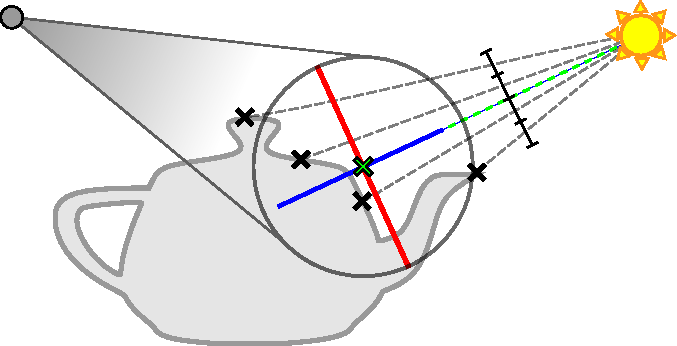
\includegraphics[width=0.7\textwidth]{shadowconetracelod.pdf}
	\caption{Shadow cone tracing from a cache (grey circle left) to a group of virtual lights (black crosses). The angle of a shadow cone depends on the sphere around the virtual lights which is the maximum of the projected sample width (red) and the depth variance (blue).} \label{fig:shadowcone}
\end{figure}
The pre-filtered depth texture is now used to estimate the angle of a cone that encloses a group of virtual lights. 
To do so, a sphere around the concerning virtual lights needs to be estimated.
\autoref{fig:shadowcone} illustrates the algorithm.
The center of the sphere (green cross in \autoref{fig:shadowcone}) is determined directly by the shadow sample position and its depth which is implicitly the average depth of all underlying virtual lights.
%Both are implicitly separate averages over all underlying virtual lights.
For the radius the maximum of two separate estimations $r_e1$ and $r_e2$ are used.
If it is assumed that depth values are normal distributed, approximately $95\%$ of all values lie within the range of two times their standard deviation (blue line in \autoref{fig:shadowcone}).
The standard deviation $\sigma$ can be easily computed:
\begin{align}
E(d) =& \frac{1}{N} \sum\limits_{i=1}^{N} d_i\\
E(d^2) =& \frac{1}{N} \sum\limits_{i=1}^{N} d_i^2\\
\sigma^2 =& E(d^2) - E(d)\\
r_e1 =& \sqrt{E(d^2) - E(d)}
\end{align}
The average depth $E(d)$ and averaged squared depth $E(d^2)$ of the virtual lights are available through the pre-filtered depth texture.

While the first estimate works well if the virtual lights have very different distances to their origin-light, it underestimates if they are parallel to the near plane of the origin-light.
Thus, the second estimate (depicted red in \autoref{fig:shadowcone}) is the size of the sample area, projected to the position of the sphere .
The sample area is determined by the relative sample size, given by the width $n_w$ and depth $n_d$ of near clip plane, the RSM resolution $R$ and the chosen Indirect Shadow LOD $l$. \todo{at some point earlier: RSM always square!}
\begin{equation}
r_e2 = E(d) \cdot \frac{n_w}{n_d \cdot R \cdot 2^{-l} }
\end{equation}

\subsubsection{Cone Trace Sampling Steps}
\begin{figure}[h]
	\centering
	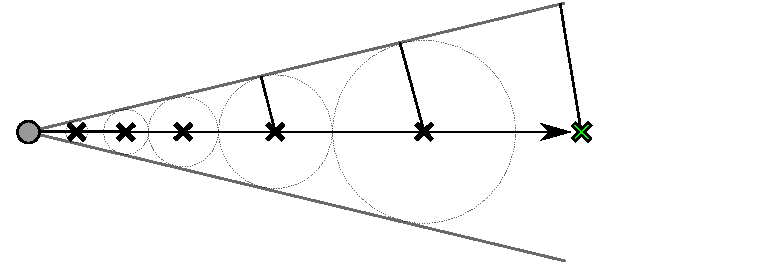
\includegraphics[width=0.7\textwidth]{conetracestep.pdf}
	\caption{Sampling a shadow cone from a cache to a light(-group). The first two enclosing circles do not touch each other because the sample distance would then below the minimum.} \label{fig:shadowconestep}
\end{figure}
The ray from cache to the sphere is sampled in increasing steps.
%Starting with a step size of one voxel width, the steps are doubled with each additional sample.
For each sample, we need to determine the mip-level in the voxel-volume of which a single voxel is approximately as large as the cone segment that is represented by the sample.
This is estimated by the radius $r_s$ of the inner circle of the current sample, as depicted in \autoref{fig:shadowconestep}.
It can be computed by easy trigonometry:
\begin{equation}
r_s = d_s \cdot \sin \alpha = d_s \cdot \frac{max(r_e1, r_e2)}{||\mathrm{p_c} - \mathrm{p_l}||}
\end{equation}
$d_s$ is the distance of the given sample to the cache. $\mathrm{p_c}$ and $\mathrm{p_c}$ are the positions of the cache and light.
Note that actual cone angle $\alpha$ does not need to be evaluated at any time.
If all values are given in voxel volume coordinates, the miplevel is simply $log_2(r_s)$.\\
The distance $d_s$ of the next sample is chosen so that two inner circles touch each other:
\begin{align}
d_{s'} =& d_s + r_s + r_{s'} = d_s + r_s + d_{s'} \cdot \sin \alpha\\
d_{s'} =& \frac{d_s + r_s}{1-\sin\alpha}
\end{align}
To avoid needless oversampling for thin cones, step sizes smaller than one voxel are no allowed (as happend between the first two samples in \autoref{fig:shadowconestep}).

Using a trilinear texture filter, the opacity values $\alpha_s$ from the voxel volume are interpolated within and across mipmap-levels.
The total visibility $V$ is accumulated front to back:
\begin{equation}
V = 1 - \sum\limits_{s=1}\alpha_s \prod\limits_{j=0}^{s-1}(1-\alpha_j)
\end{equation}
The sampling stops if either the light group position is reached or the visibility approaches zero.

\section{Cache Interpolation}
After all caches have been populated with lighting data, their information needs to be interpolated across the screen.

As in the cache allocation pass, each pixel uses its world position to compute its eight nearest caches.
For the diffuse lighting, the irradiance Spherical Harmonic is evaluated with the per-pixel normal in each cache.
The result is bilinear interpolated depending on the relative position of the pixel to its eight nearest caches.
To retrieve the final visible radiance, the interpolated radiance value is then multiplied with the diffuse BRDF.

For the specular lighting we need to determine the relative coordinate and, depending on the Blinn-Phong exponent, at which mipmap-level the Specular Environement Map of each cache should be sampled.
Identical to the computation of the Specular Environment Map, finding the coordinate involves the projection of the normal vector using a local view space (see \autoref{sec:impl:specenvmap}).
Since the direction to the camera from cache to cache is almost the same, we transform the per-pixel normal only to its own local view space.
This introduces a slight inaccuracy but circumvents the possibility that a normal vector might lie outside of a cache's local view hemisphere.\\
The mipmap-level is computed similar as $\gamma_{max}$ before, only that this time the mipmap-level $m$ is searched for.
\begin{align}
\int\limits_{2\pi sr} (\cos\theta)^{\gamma}  \,\mathrm{d}\omega = \frac{2\pi}{(R \cdot 2^{-m})}\\
m = \log_2 \Big(\frac{2 \cdot R^2}{\gamma + 1} \Big) \cdot \frac{1}{2}
\end{align}
where $R$ is the resolution of a single Specular Environment Map.
As before with the diffuse lighting, the results of all caches are bilinear interpolated and multiplied with the specular reflectivity of the corresponding pixel.

Pixels in transition areas (see \autoref{sec:impl:cavcascading}) compute two radiance values, one for both CAV cascade.
The results are interpolated linearly.

\section{Implementation}
\emph{As many as possible details should be delayed into this chapter. If it gets large or starts to mirror the main part, make it a chapter!}

This is the right place for describing how to use Compute, OpenGL etc. for achieving the rather abstract formulated goals of the sections before.

Deferred Renderer, 32bits per Layer RGB(A) srgb - Diffuse, RG 16snorm - Normals with angles, extra infos todo, R32F Depth Buffer (swapped near/far)\\
(This detail belongs more or less to Eva...)

\subsection{Direct Lighting}
Uses also Blinn-Phong.

\subsection{Cache Allocation} \label{sec:impl:cachealloc}
cacheList via shared memory etc.
"Adress Coord Cache"

\subsection{Indirect Lighting}

Traverse in Morton Order.

\subsubsection{Voxelization}
This can be done very fast using the GPU.
We use the conservative voxelization algorithm described by Crassin and Green in "OpenGL Insights" \cite{bib:openglinsightsvoxel}.
On more recent hardware conservative voxelization is supported directly

\subfilebib % Makes bibliography available when compiling as subfile
\end{document}